\section{Specific Requirements}\label{sec requirements}

\subsection{External Interface Requirements}

\subsubsection{User interfaces}

The user interfaces must satisfy the following UI constraints:
\begin{itemize}
	\item Web application
	\begin{enumerate}
		\item The web pages must adhere to the W3C standards. In particular, the software shall conform to the HTML~5~\cite{w3c-html5}, CSS~\cite{w3c-css} standards.
	\end{enumerate}
	\item Mobile application
	\begin{enumerate}
		\item The iOS version must adhere to the iOS Human Interface Guidelines~\cite{apple-ios-hig}.
		\item The Android version must follow Android design guidelines~\cite{google-android-hig}.
	\end{enumerate}
		\item Common to web and mobile applications:
		\begin{enumerate}
			\item The client applications must have an UI that is accessible to disabled people.
			\item The interface must offer the possibility to choose the language used at all times.
			\item The first screen(homepage) must ask the guest to log in or sign up in order to begin operations.
			\item Once logged, the homepage must show the vehicle search page.
			\item UI controls and views must be suitable for the input interface and the screen size.
		\end{enumerate}
	\item Vehicle application
	\begin{enumerate}
		\item Radio and navigator applications must be implemented.
		\item A Label on the screen will always notify the driver about the current charges.
	\end{enumerate}
	\item Server back-end
	\begin{enumerate}
		\item The server back-end must be configurable by means of a configuration text file.
	\end{enumerate}
	
\subsubsection{Hardware interfaces}
The embedded system of any vehicles must be provided of	
\begin{itemize}
	\item a 7" touchscreen display
	\item a GPS device
	\item sensors that check if all the parts of the car are working correctly
	\item sensors that check how many passengers are on the car
	\item a 4G router for a stable Internet connection
	\item a secondary battery used only if the main battery is discharged. The vehicle can't use this battery
\end{itemize}

\subsubsection{Software interfaces}
The required software products used by the back-end are:
\begin{itemize}
	\item MySQL 5.7\footnote{\url{http://dev.mysql.com}}
	\item Java SE 8\footnote{\url{http://www.oracle.com/technetwork/java/javase/overview/index.html}}
\end{itemize}
The required software product used by the car application is:
\begin{itemize}
	\item Java Embedded\footnote{\url{http://www.oracle.com/technetwork/java/embedded/overview/index.html}}
\end{itemize}
The required operating systems for the mobile application atr:
\begin{itemize}
	\item iOS 8 or more recent
	\item Android 6.0 or more recent
\end{itemize}

For a detailed specification of the programmatic interfaces, see \autoref{sec:api}.
	
\subsubsection{Communications interfaces}
The clients communicate with the server via HTTPS requests (port 443).

\end{itemize}

\subsection{System Features}

\subsubsection{Driver registration}

\subsubsubsection{Purpose}
Any guest can subscribe through web or mobile applications.

In both cases the guest has to fill a registration form and must agree to the personal data policy according to his/her country privacy laws, otherwise the registration request shall be aborted.

As soon as the guest has submitted all the data, the system verifies the consistency of the information and a confirmation mail with a password is sent to the email address indicated in the registration form. The guest 
must confirm his/her email address for end the registration.

Once registered a guest can be recognized as a driver through the login phase.

\subsubsubsection{Scenario 1}
Bob, a normal citizen without a car, has just discovered the existence of the PowerEnJoy Service and he wants to use it.

He opens the homepage of PowerEnJoy website and procedes to the registration clicking on the button "Signup".

He gives all the information required and authorises the personal data treatment. 

The system verifies all the information that bob submitted to the form and sends a confirmation mail to him.

Bob checks his mailbox, opens the mail and clicks on "Confirm email". He is also notified about his current password.

The system informs Bob that he is successfully registered.

\begin{figure}[H]
	\centering
	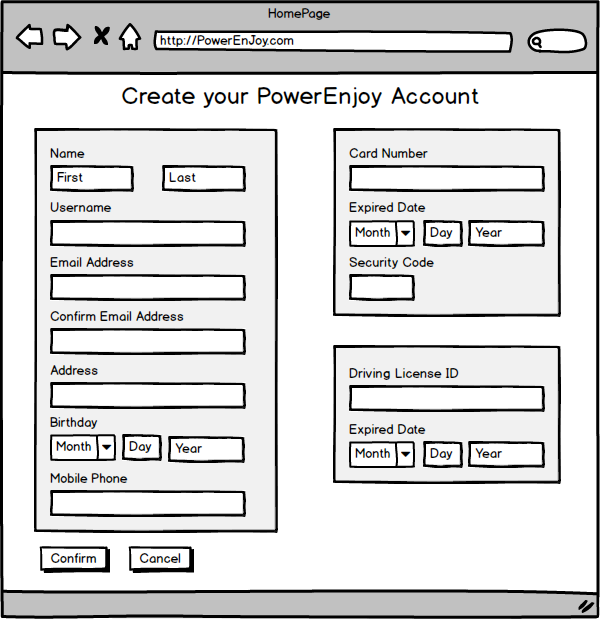
\includegraphics[width=\textwidth]{mockup/WebRegistration.png}
	\caption{Concept of the registration webpage.}
\end{figure}

\begin{figure}[H]
	\centering
	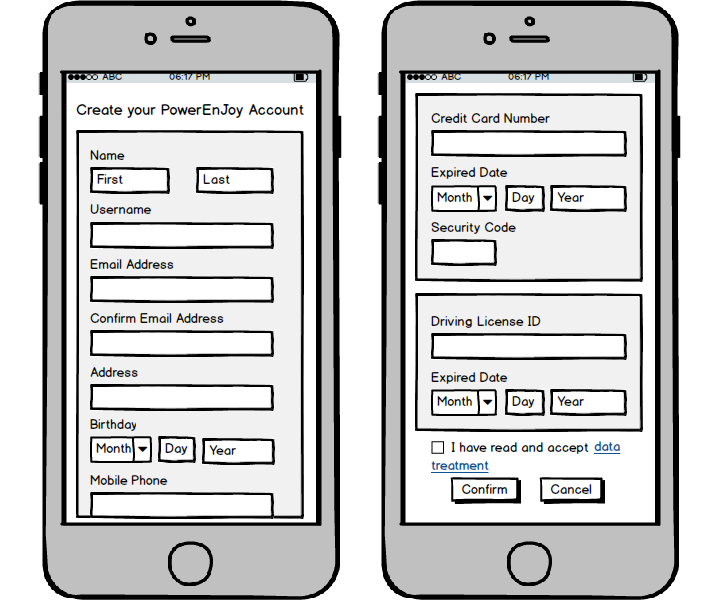
\includegraphics[width=\textwidth]{mockup/MobileRegistration.png}
	\caption{Concept of the mobile registration page.}
\end{figure}

\subsubsubsection{Use case description and sequence diagram}

\begin{table}[H]
\begin{center}
	\begin{tabular}{| l | p{0.6\textwidth} |}
		\hline
		Actor & Guest \\
		\hline
		Goal & G3
		\\
		\hline
		Input condition & The guest chooses to create a new driver account.  \\
		\hline
		Event Flow & \begin{enumerate}
			\item The registration form is loaded and the guest compiles it.
			\item The guest authorizes the personal data treatment.
			\item The guest clicks on "Confirm".
			\item The system sends a confirmation email.
			\item The guest reads the e-mail, with his/her password, received by PowerEnJoy and clicks on the link to confirm the registration.
		\end{enumerate}
		\\
		\hline
		Output condition & The system tells the guest that he/she has been successfully registered. \\
		\hline
		
		Exception &  \begin{itemize}
			\item Some exceptions are handled notifying the guest of the problem through a dynamic message box or reloading the registration form.
			
			The requirements that generate these kind of exceptions are:
			\ref{f-sameinfo},   %The username/e-mail is already used by someone else.
			\ref{f-samelicense}, %The driving license is already used by someone else.
			\ref{f-usrn},       %The username doesn't respect the restrictions.
			\ref{f-wrongmail},  %The emails are not equals.
			\ref{f-licenseexp}, %The driving license is expire
			\ref{f-cc}.			%The payment method is not valid.
			
			\item Some exceptions are handled aborting the registration (all guest's data are deleted).
			
			The requirements that generate these kind of exceptions are:
			\ref{f-dataTreat},   %The user doesn't authorises the data treatment.
			\ref{f-confirm}.   %The user doesn't confirms the registration clicking on the link received via e-mail.
		\end{itemize}
		\\
		\hline
	\end{tabular}
\end{center}
\end{table}

\begin{figure}[H]
	\begin{center}
		\centering
		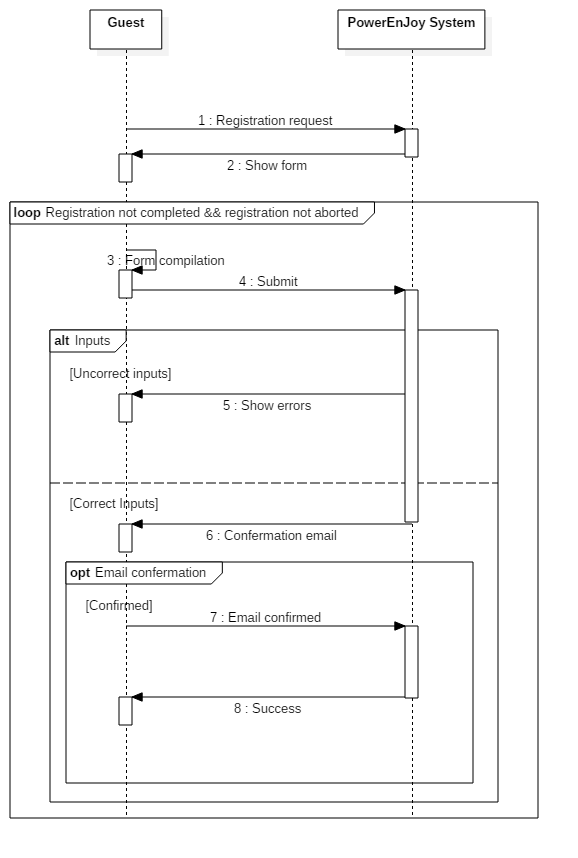
\includegraphics[height=0.9\textheight, keepaspectratio]{sequence_diagram/Registration.jpg}
		\caption{Sequence diagram of the registration process.}
	\end{center}
\end{figure}

\subsubsubsection{Associated functional requirements}

\begin{enumerate}
	\item Guests must provide the following information:
	\begin{itemize}
		\item name
		\item surname
		\item username
		\item email address
		\item address
		\item birthday
		\item phone number
		\item credit card number
		\item credit card expire date
		\item credit card security code
		\item driving license ID
		\item driving license expired date	
	\end{itemize}
	\item There mustn't be another user already subscribed with the same username or e-mail. \label{f-sameinfo}
	\item There mustn't be another driver already subscribed with the same driving license. \label{f-samelicense}	
	\item Username must match the regular expression\\``\texttt{[a-zA-Z][a-zA-Z0-9]\{2,20\}}''    \label{f-usrn}
	\item The system accepts the email only if it is entered identically both times.\label{f-wrongmail}
	\item The driving license must be valid and not expired.
	\label{f-licenseexp}
	\item The payment method must be valid and not expired.
	\label{f-cc}
	\item If the personal data treatment is not authorised, the subscription is canceled. \label{f-dataTreat}
	\item The system must allow the guest to abort the registration process at any time.
	\item Email confirmation process:
	\begin{enumerate}
		\item The subscription ends successfully when the guest clicks on the link in the confirmation email. The system will provide, through the mobile or the web application, a password for the new driver.
		\item After one day without an answer, the guest's registration info are deleted and the guest may re-try the registration process.  \label{f-confirm}
	\end{enumerate}
\end{enumerate}

\subsubsection{Search and reservation}

\subsubsubsection{Purpose}
Any logged driver, in possession of a valid driving license and a regular status of payments, can search and reserve a vehicle through the web application or the mobile app.

The system shows him/her a map, of the area nearby the driver, with the available vehicles as colorful markers. There are 3 diffent colors for the markers:
\begin{itemize}
	\item red: 50-75\% of the battery empty
	\item yellow: 25-50\% of the battery empty
	\item green: 0-25\% of the battery empty
\end{itemize}
The driver can also search vehicles nearby from a given address through a search box on the page.

Once the driver chooses the vehicle he can click on its marker and a new dynamic frame will show more information about the vehicle and the possibility to reserve it clicking on the button "Reserve".
The system notifies the driver that he/she succesfully reserved a vehicle.

Vehicles with more than 75\% of the battery empty require assistance from the operators to be recharged and the system won't show them as available. 


\subsubsubsection{Scenario 1}
Bob logs in the PowerEnJoy application through his web browser. He wants to reserve a vehicle because an important meeting is waiting for him. Once logged the system redirects him to the homepage that now shows the vehicle search page. Bob realizes there's only a vehicle with a red marker within 1km from him. Bob has to hurry up so he clicks on the red marker and than on the button "Reserve".

\subsubsubsection{Scenario 2}
Alice logs in the PowerEnJoy application through his mobile phone. She wants to reserve a vehicle but everytime she clicks on the button "Reserve" of an available vehicle the system stops her showing a dynamic message box that remember her to solve her pending payments. Once alice solves her pending payments she will be able to reserve an available vehicle.

\begin{figure}[H]
	\centering
	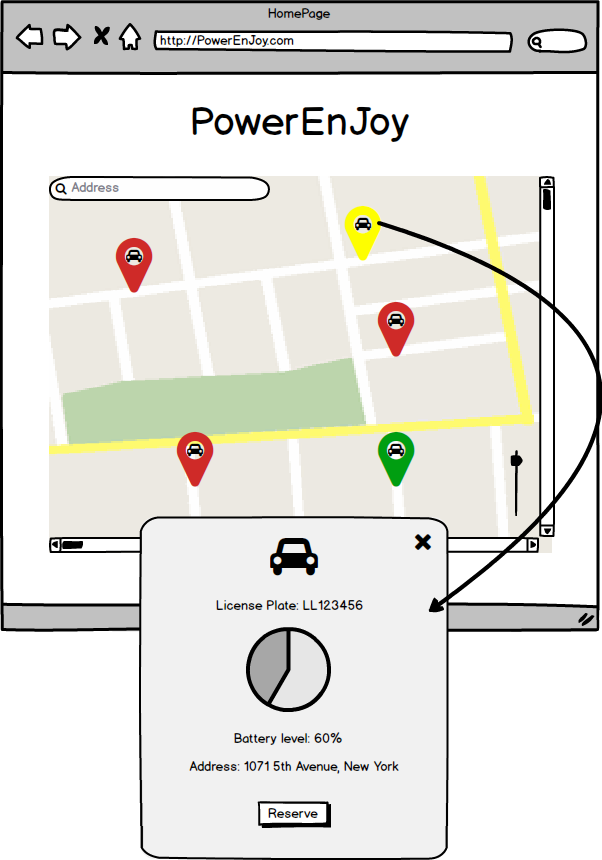
\includegraphics[width=\textwidth]{mockup/WebSearch.png}
	\caption{Concept of the search webpage.}
\end{figure}

\begin{figure}[H]
	\centering
	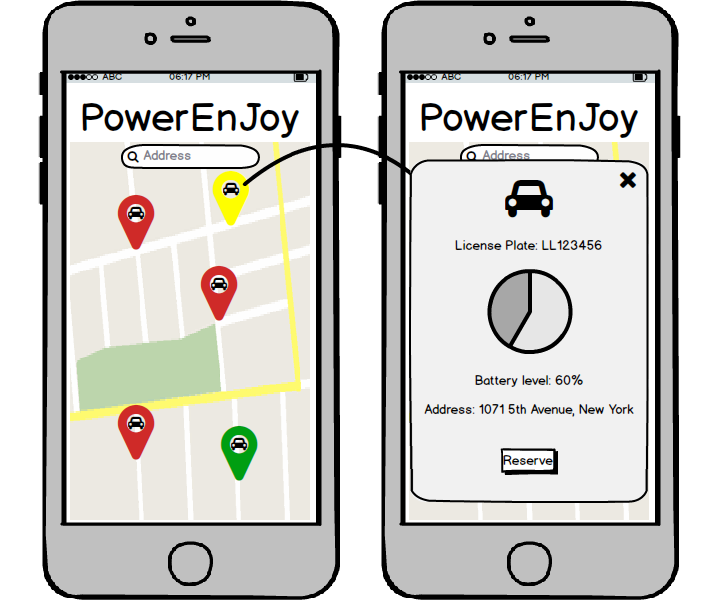
\includegraphics[width=\textwidth]{mockup/MobileSearch.png}
	\caption{Concept of the mobile search page.}
\end{figure}

\subsubsubsection{Use case description and sequence diagram}

\begin{table}[H]
	\begin{center}
		\begin{tabular}{| l | p{0.6\textwidth} |}
			\hline
			Actor & Driver \\
			\hline
			Goal & G1.1
			\\
			\hline
			Input condition & The driver is already logged and chooses to reserve a vehicle.  \\
			\hline
			Event Flow & \begin{enumerate}
				\item The driver opens the home page and search an available vehicle.
				\item Once choosen, the driver clicks on "Reserve".
			\end{enumerate}
			\\
			\hline
			Output condition & The system notifies the driver that he/she succesfully reserved the choosen vehicle \\
			\hline
			
			Exception &  \begin{itemize}
				\item Some exceptions are handled notifying the driver of the problem through a dynamic message box.				
				The requirements that generate these kind of exceptions are:
				\ref{f-expired},    %The driving license is expired.
				\ref{f-regular},    %Status of payments is not regular.			
				\item No vehicle is available in the driver's area.
				\end{itemize}
			\\
			\hline
		\end{tabular}
	\end{center}
\end{table}

\begin{figure}[H]
	\begin{center}
		\centering
		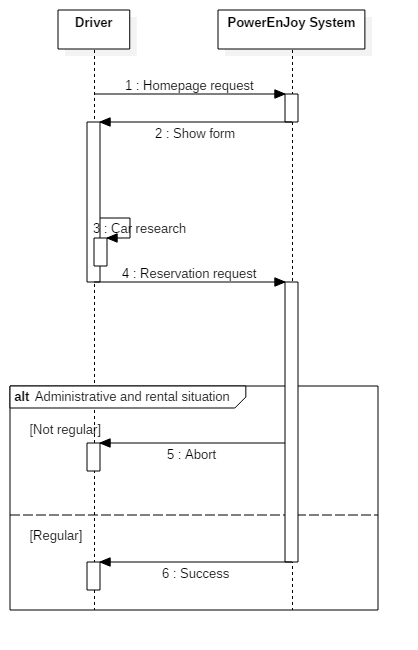
\includegraphics[height=0.9\textheight, keepaspectratio]{sequence_diagram/SearchReservation.png}
		\caption{Sequence diagram of search and reservation process.}
	\end{center}
\end{figure}

\subsubsubsection{Associated functional requirements}

\begin{enumerate}
	\item The driver must be logged in order to search and reserved a vehicle.
	\item The system must show to the driver a map of the area, within a range of 1km from him/her or from a given address, with the available vehicles.
	\item The system must provide more information about an availabe vehicle. These information are
		\begin{itemize}
			\item license plate
			\item address
			\item battery level
		\end{itemize}
	\item The system must allow a driver to reserve an available vehicle.
	\item In order to reserve a vehicle the driver's driving license mustn't be expired. \label{f-expired}
	\item In order to reserve a vehicle the driver's status of payments must be regular. \label{f-regular}
	\item The system must prevent the driver from reserving more than one vehicle at time.
	\item The system must prevent the driver from reserving a vehicle already reserved, or in use, by another driver.
	\item The system must prevent the driver from reserving an out of service or a discharged vehicle.
	\item After a reservation is 
\end{enumerate}

\subsubsection{Vehicle use}

\subsubsubsection{Purpose}
The driver can use the vehicle after he/she reserved it.

When the driver is nearby the reserved vehicle he/she can click on the button "I'm nearby" and the system will check the GPS signal of both the vehicle and the driver's mobile phone, to assess if they are within a 25 meters range. If they are within that range, the system will unlock the vehicle and the driver can enter. This operation is available only through the mobile application.

As soon as the engine ignites, the system starts charging the driver for a given amount of money per minute; the driver is notified of the current charges through a screen on the vehicle.

\subsubsubsection{Scenario 1}
Bob has already reserved a vehicle and he is going to pick it up. He is far about 50 meters from the vehicle and he clicks on the button "I'm nearby" of the mobile application. The system checks the GPS signal of both the vehicle and the Bob's mobile phone, and it doesn't unlock the vehicle notifing Bob that he's too far from it.

Once Bob is in front of the vehicle he clicks again on "I'm nearby", the system unlocks the vehicle and he finally enter.

Bob starts the vehicle and the system notifies him about his current charges thanks to the vehicle application. He can start his ride.

\begin{figure}[H]
	\centering
	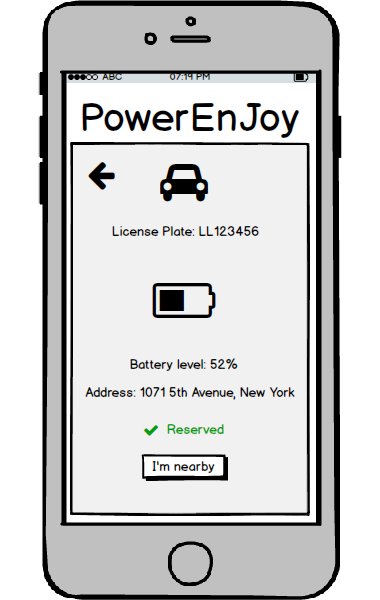
\includegraphics[height=20cm]{mockup/MobileUnlock.png}
	\caption{Concept of the mobile vehicle unlock page.}
\end{figure}

\begin{figure}[H]
	\centering
	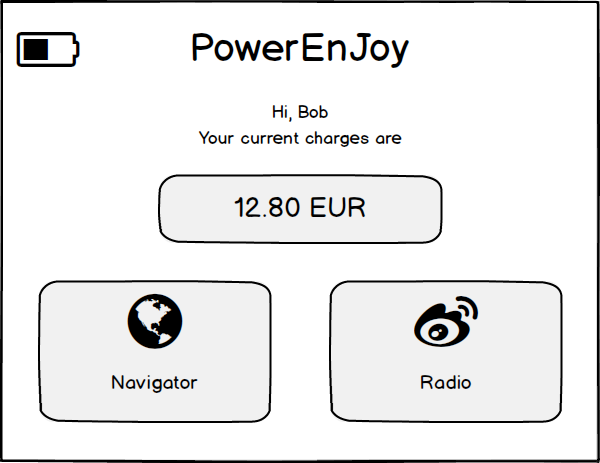
\includegraphics[width=\textwidth]{mockup/VehicleApplication.png}
	\caption{Concept of the vehicle application.}
\end{figure}

\begin{table}[H]
	\begin{center}
		\begin{tabular}{| l | p{0.6\textwidth} |}
			\hline
			Actor & Driver \\
			\hline
			Goal & G1.2
			\\
			\hline
			Input condition & The driver has already reserved a vehicle and he/she is going to pick it up.  \\
			\hline
			Event Flow & \begin{enumerate}
				\item The driver is within 25 meters from the vehicole.
				\item The driver opens the reservation mobile page, through a section of the homepage, and clicks on "I'm nearby".
				\item The system unlocks the vehicle.
				\item The driver enters and starts the vehicle. 
			\end{enumerate}
			\\
			\hline
			Output condition & The driver starts his/her ride and the system keeps notifying him/her about his/her current charges. \\
			\hline
			
			Exception &  \begin{itemize}
				\item Some exceptions are handled notifying the driver of the problem through a dynamic message box.				
				The requirements that generate these kind of exceptions are:
				\ref{f-reservationcanc},    %It passed more than one hour from the reservation
				\ref{f-nearby},    %The driver isn't nearby.			
			\end{itemize}
			\\
			\hline
		\end{tabular}
	\end{center}
\end{table}

\begin{figure}[H]
	\begin{center}
		\centering
		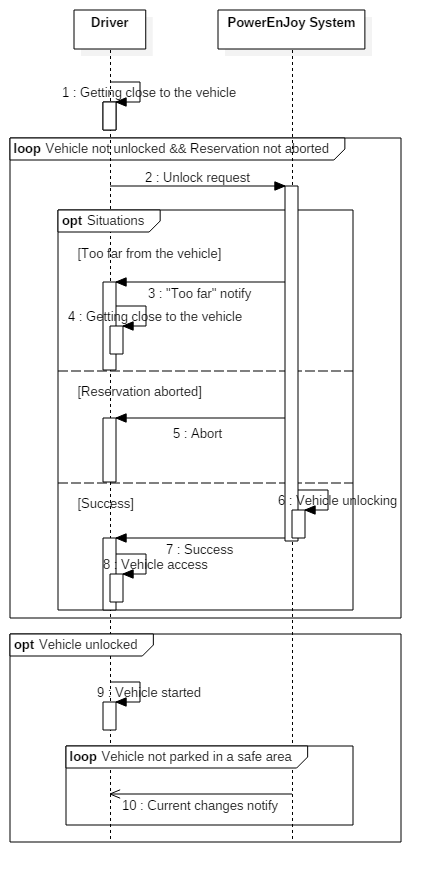
\includegraphics[height=0.9\textheight, keepaspectratio]{sequence_diagram/Unlock.png}
		\caption{Sequence diagram of the vehicle use process.}
	\end{center}
\end{figure}

\subsubsubsection{Associated functional requirements}

\begin{enumerate}
	\item It mustn't pass more than one hour from the reservation to the 
	unlocking of the vehicle. \label{f-reservationcanc}
	\item The driver must be within 25 meters from the vehicle to unlock it. \label{f-nearby}
\end{enumerate}

\subsubsection{Vehicle parking}

\subsubsubsection{Purpose}

Once the driver has finished to use the vehicle he/she should be able to park it in safe areas provided by the system. These areas are displayed by the navigator vehicle application.



\subsection{Performance Requirements}

\subsection{Software System Attributes}

\subsection{Alloy}